\section{Программная реализация методов моделирования процессов цифрового документооборота}

\section{Технологическая часть}
\subsection{Реализация алгоритма моделирования с помощью sTPN}

Для построения сети Петри и дальнейшей обработки результатов моделирования было выбрано программное обеспечение OrisTool\cite{oris}. Данное ПО обладает всеми необходимыми для решения поставленной задачи функциями:

\begin{itemize}
	\item возможность построения стохастической сети Петри;
	\item возможность проведения моделирования сети Петри;
	\item наличие прямого и обратного переходного анализа;
	\item визуализация полученных данных.
\end{itemize}

\subsection{Сопоставление BPMN 2.0 и сетей Петри}

Для корректного построения модели необходимо установить связь между элементами BPMN 2.0 с сетями Петри. Сопоставление представлено на рисунке \ref{fig:mapping}.

\begin{figure}[h!btp]
	\centering
	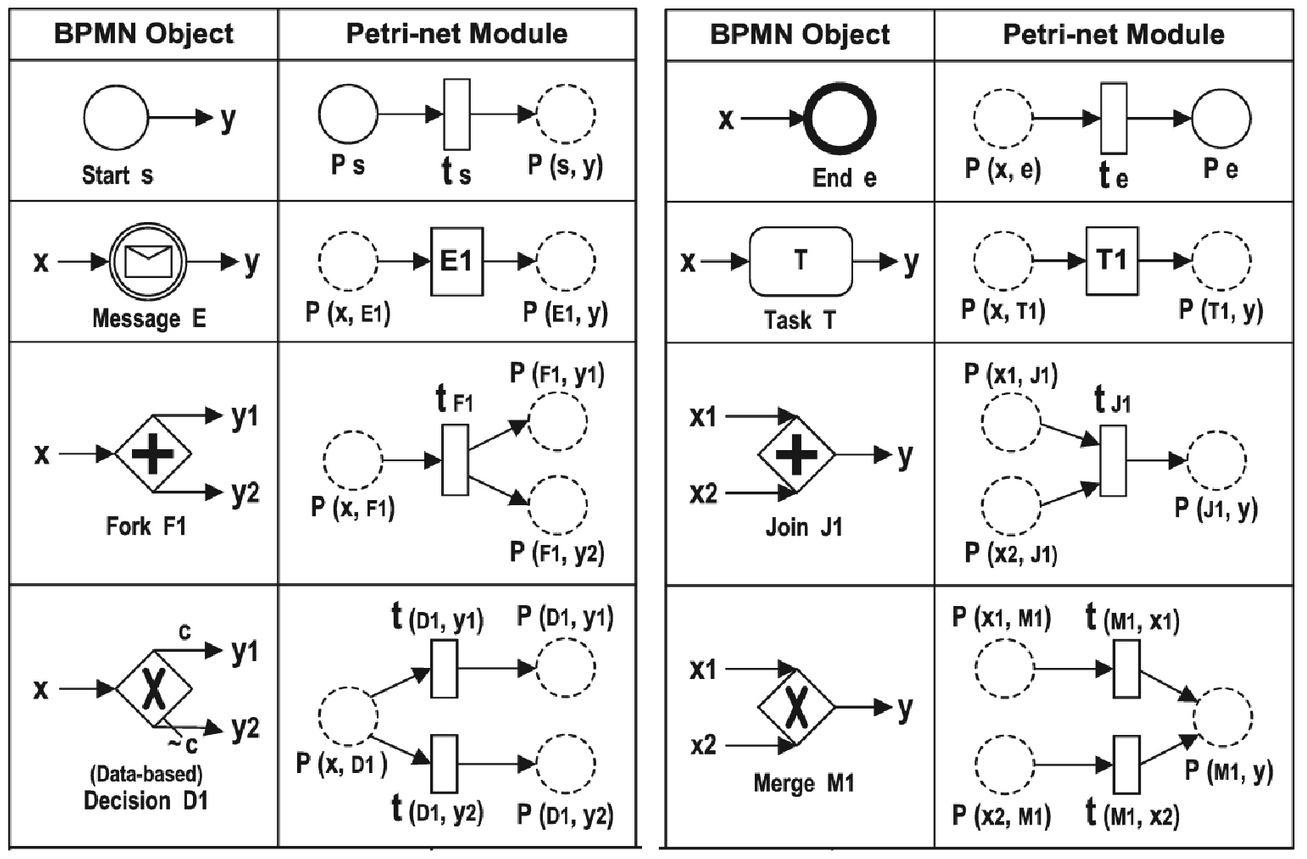
\includegraphics[width=0.75\textwidth]{../inc/mapping.png}
	\caption{Сопоставление BPMN 2.0 и сетей Петри}
	\label{fig:mapping}
\end{figure}


\subsection{Реализация алгоритма квантового моделирования}

\subsubsection{Выбор и обоснование средств разработки}

В качестве языка программирования был выбран логический язык \texttt{SWI-Prolog}\cite{prolog} -- инструмент для работы с логическим программированием, предназначенный для поиска заданного решения. Для решения поставленной задачи данный язык программирования обладает следующими достоинствами:

\begin{itemize}
	\item декларативный подход: в отличие от императивных языков программирования, \texttt{SWI-Prolog} позволяет описывать задачи и решения в декларативной форме -- что должно быть сделано, а не как именно это нужно выполнить;
	
	\item управление перебором: эффективное управление процессом перебора возможных решений (англ. \texttt{backtracking}) позволяет оптимально находить все возможные решения для заданной проблемы, автоматически пробуя различные варианты и отсекая неверные пути;
	
	\item встроенные предикаты: \texttt{SWI-Prolog }предлагает обширную библиотеку встроенных предикатов для различных математических операций, что упрощает реализацию многих стандартных математических функций и операций;
	
	\item работа с символическими выражениями: возможность обрабатывать и вычислять символические выражения, позволяет отказаться от полного числового ввода, что полезно для математических формул, требующих символического вывода, а не только численного решения;
	
	\item интеграция с другими языками и системами: данный языка возможно интегрировать с другими языками программирования, такими как \texttt{Python} или \texttt{C}, что позволяет использовать \texttt{SWI-Prolog} для логических и символических вычислений в рамках более крупных систем;
	
	\item отладка и разработка: \texttt{SWI-Prolog} предлагает различные инструменты для отладки и трассировки программ, что помогает в разработке сложных алгоритмов и облегчает поиск и исправление ошибок.
\end{itemize}

\subsubsection{Листинги кода}

Реализация программы для подсчёта вероятности прохождения документа из начального статуса в финальный и поиска данного статустного пути, без учёта базы знаний, представлена в листинге \ref{code:prog}.

\begin{lstlisting}[label=code:prog, caption={Реализация поиска пути и вероятности}]
transition_probability(EFT, LFT, Probability) :-
  Probability is (LFT - EFT) / LFT.

find_path(Start, End, Path, Probability, Steps) :-
  travel(Start, End, [Start], 1, 0, RevPath, Probability, Steps),
  reverse(RevPath, Path).

travel(Start, End, Visited, CurrentProb, CurrentSteps, [End|Visited], FinalProb, FinalSteps) :-
  transition(Start, End, EFT, LFT),
  transition_probability(EFT, LFT, StepProb),
  FinalProb is CurrentProb * StepProb,
  FinalSteps is CurrentSteps + 1.

travel(Start, End, Visited, CurrentProb, CurrentSteps, Path, FinalProb, FinalSteps) :-
  transition(Start, Mid, EFT, LFT),
  Mid \= End,
  \+member(Mid, Visited),
  transition_probability(EFT, LFT, StepProb),
  NewProb is CurrentProb * StepProb,
  NewSteps is CurrentSteps + 1,
  travel(Mid, End, [Mid|Visited], NewProb, NewSteps, Path, FinalProb, FinalSteps).
\end{lstlisting}

Реализация программы для нахождения вероятностного распределения представлена в листинге \ref{code:prog2}.

\clearpage

\begin{lstlisting}[label=code:prog2, caption={Реализация построения вероятностного распределения}]
	initial_distribution(["status1"-p1, "status2"-p2]).
	
	update_distribution(Dist, NewDist) :-
	  findall(S-NewProb, (
	    member(S-_, Dist),
	    findall(P, (
	      member(S1-P1, Dist),
	      transition(S1, S, EFT, LFT),
	      P is (EFT / LFT) * P1
	    ), Probs),
	    sum_list(Probs, TotalProb),
	    NewProb is TotalProb
	  ), TempDist),
	  normalize_distribution(TempDist, NewDist).
	
	normalize_distribution(Dist, Normalized) :-
	  sum_list(Dist, Total, 0),
	  maplist(normalize_prob(Total), Dist, Normalized).
	
	normalize_prob(Total, S-P, S-NormP) :- NormP is P / Total.
	
	sum_list([], Total, Total).
	sum_list([_-P|T], Total, Acc) :- NewAcc is Acc + P, sum_list(T, Total, NewAcc).
	
	perform_steps(Dist, 0, [Dist]).
	perform_steps(Dist, N, [Dist|Rest]) :-
	  N > 0,
	  update_distribution(Dist, NewDist),
	  M is N - 1,
	  perform_steps(NewDist, M, Rest).
	
	print_numeric_results([]).
	print_numeric_results([H|T]) :-
	  findall(Prob, member(_-Prob, H), Probs),
	  writeln(Probs),
	  print_numeric_results(T).

\end{lstlisting}

\pagebreak
